\documentclass[a4paper]{article}
\usepackage[margin=2.5cm]{geometry} % Standard page layout
\usepackage{pgfplots}
\usepackage{booktabs} % For nice tables
\pgfplotsset{compat=1.18}
\usepgfplotslibrary{statistics} % Required for box plots
\usepackage[utf8]{inputenc} % Character support
\usepackage[T1]{fontenc} % For font encoding, helps with code snippets
\usepackage{hyperref} % For clickable links
\usepackage{url} % For formatting URLs
\usepackage{listings} % For code snippets
\usepackage{xcolor} % For code snippet colors

% Define a custom python style for lstlistings
\definecolor{codegreen}{rgb}{0,0.6,0}
\definecolor{codegray}{rgb}{0.5,0.5,0.5}
\definecolor{codepurple}{rgb}{0.58,0,0.82}
\definecolor{backcolour}{rgb}{0.95,0.95,0.92}

\lstdefinestyle{mystyle}{
    backgroundcolor=\color{backcolour},   
    commentstyle=\color{codegreen},
    keywordstyle=\color{magenta},
    numberstyle=\tiny\color{codegray},
    stringstyle=\color{codepurple},
    basicstyle=\ttfamily\footnotesize,
    breakatwhitespace=false,         
    breaklines=true,                 
    captionpos=b,                    
    keepspaces=true,                 
    numbers=left,                    
    numbersep=5pt,                  
    showspaces=false,                
    showstringspaces=false,
    showtabs=false,                  
    tabsize=2
}

\lstset{style=mystyle}

\title{Analysis and Benchmarking of Matrix Multiplication Implementations}
\author{Cristian Romeo}
\date{\today}

\begin{document}

\maketitle

\section{Introduction}
Matrix multiplication is a fundamental operation in scientific computing, machine learning, and data analysis. The performance of this calculation can vary drastically based on the programming language, algorithm implementation, and underlying hardware architecture.

The objective of this study is to analyze the performance of a matrix multiplication operation and, more importantly, to demonstrate the process of building a reliable test harness to obtain meaningful measurements. I will start by analyzing a simple Python implementation and evolve it into a structured benchmark framework, which is then used to compare the initial implementation with the refactored one.

\section{Methodology and Code Improvement}
The source code for this project is available on GitHub: \url{https://github.com/cristianromeo/task-1.-language-benchmark-of-matrix-multiplication}.

\subsection{Initial Implementation ('matrix.py')}
The first version of the code, contained in \texttt{matrix.py}, had several issues that prevented accurate benchmarking:
\begin{itemize}
    \item It was a monolithic script that mixed data generation, calculation logic, and time measurement.
    \item The matrix size was hard-coded to \texttt{n=1024}.
    \item It performed only a single measurement, making the results highly susceptible to momentary fluctuations in CPU or system load.
    \item It contained a critical bug in the innermost loop (\texttt{C[i][j] += A[i][k] * B[k][k]} instead of \texttt{B[k][j]}), which not only produced an incorrect result but also altered the memory access pattern.
\end{itemize}

A snippet from \texttt{matrix.py} shows these issues:
\begin{lstlisting}[language=Python, caption={Snippet from the initial 'matrix.py'}]
import random
from time import *

n = 1024 # Hard-coded size

A = [[random.random() for _ in range(n)] for _ in range(n)]
B = [[random.random() for _ in range(n)] for _ in range(n)]
C = [[0 for _ in range(n)] for _ in range(n)]

start = time() # Single time measurement

for i in range(n):
    for j in range(n):
        for k in range(n):
            C[i][j] += A[i][k] * B[k][k] # Buggy logic

end = time()

print("%.6f" % (end-start))
\end{lstlisting}

\subsection{Refactored Benchmark Harness}
To address these limitations, I reorganized the code into a robust benchmark harness, following software engineering best practices.

\subsubsection{Separation of Production and Test Code}
The first step was to separate responsibilities. The pure multiplication logic was moved into an importable module (\texttt{code/python/matrix\_mul.py}). This module contains only the functions for creating and multiplying matrices.

\begin{lstlisting}[language=Python, caption={Snippet from the refactored 'matrix\_mul.py'}]
# Production code: matrix_mul.py
from typing import List, Optional
import random

Matrix = List[List[float]]

def random_matrix(n: int, seed: Optional[int] = None) -> Matrix:
    # ... implementation ...

def zeros_matrix(n: int) -> Matrix:
    return [[0.0 for _ in range(n)] for _ in range(n)]

def multiply(A: Matrix, B: Matrix, order: str = "ikj") -> Matrix:
    n = len(A)
    C = zeros_matrix(n)

    if order == "ikj":
        for i in range(n):
            Ai = A[i]
            # ... correct logic ...
    elif order == "ijk":
        # ... correct logic ...
    # ... other orders ...
    else:
        raise ValueError(f"Unknown order: {order}")

    return C
\end{lstlisting}

Two separate scripts now use this module:
\begin{enumerate}
    \item \textbf{Correctness Tests (\texttt{code/python/tests/test\_matrix.py}):} Uses the \texttt{unittest} framework to verify that the algorithm produces mathematically correct results.
    \item \textbf{Performance Tests (\texttt{code/python/benchmark.py}):} Is dedicated exclusively to measuring the execution time of the multiplication function.
\end{enumerate}

\subsubsection{Calculation Parametrization}
Unlike the original script, \texttt{benchmark.py} uses Python's \texttt{argparse} library to accept command-line parameters. This is essential for scientific analysis, allowing the user to specify:
\begin{itemize}
    \item The matrix size (\texttt{--n}).
    \item The loop order (\texttt{--order}, e.g., "ikj", "ijk", "kij").
    \item The number of runs (\texttt{--runs}).
    \item A random seed (\texttt{--seed}) for reproducibility.
\end{itemize}

\begin{lstlisting}[language=Python, caption={Argument parsing in 'benchmark.py'}]
import argparse
import time
import statistics
from matrix_mul import random_matrix, multiply

def main():
    parser = argparse.ArgumentParser(description="Matrix multiplication benchmark (pure Python)")
    parser.add_argument("--n", type=int, default=256, help="matrix size n (n x n)")
    parser.add_argument("--runs", type=int, default=3, help="number of timed runs")
    parser.add_argument("--order", type=str, default="ikj", help="loop order: ikj, ijk, ...")
    parser.add_argument("--seed", type=int, default=None, help="random seed (None = random)")
    args = parser.parse_args()
    # ... benchmark logic follows ...
\end{lstlisting}

This flexibility is crucial for testing different hypotheses, such as the impact of loop order on cache utilization.

\subsubsection{Multiple Runs for Statistical Reliability}
A single time measurement is not reliable. The benchmark harness solves this by accepting the \texttt{--runs} argument. The script runs the calculation multiple times, storing the time for each execution. At the end, it calculates and reports fundamental aggregate statistics like the \textbf{mean}, \textbf{median}, and \textbf{standard deviation}. The median, in particular, is a robust metric for typical performance as it is less affected by random outliers.

\section{Benchmarking Process}
The analysis presented in this document focuses on the comparison of the two Python implementations. Both versions were tested on the same machine to ensure consistent hardware conditions. I used the following command:

\texttt{python benchmark\_script.py --n 256 --runs 100 --order ikj}

I chose a matrix size of \texttt{n=256} and ran the experiment 100 times for each script to gather a stable statistical sample. The \texttt{ikj} loop order was used for both tests for a direct comparison.

\section{Results and Analysis}
The results of the 100 tests for each implementation are summarized in Table \ref{tab:python_summary_comparison} and visualized in the box plot in Figure \ref{fig:python_benchmark_comparison}.

% --- COMPARISON SUMMARY TABLE ---
\begin{table}[h!]
    \centering
    \begin{tabular}{lrr}
        \toprule
        \textbf{Statistic} & \textbf{matrix\_mul.py} & \textbf{Buggy 'matrix.py'} \\
        \midrule
        Runs   & 100        & 100        \\
        Mean   & 1.511969 s & 2.343269 s \\
        Median & 1.530636 s & 2.282895 s \\
        StdDev & 0.384953 s & 0.289646 s \\
        Min    & 0.988593 s & 1.897993 s \\
        Max    & 2.677320 s & 3.316186 s \\
        \bottomrule
    \end{tabular}
    \caption{Summary comparison of Python benchmark results (n=256).}
    \label{tab:python_summary_comparison}
\end{table}

% --- COMPARISON BOX PLOT ---
\begin{figure}[h!]
    \centering
    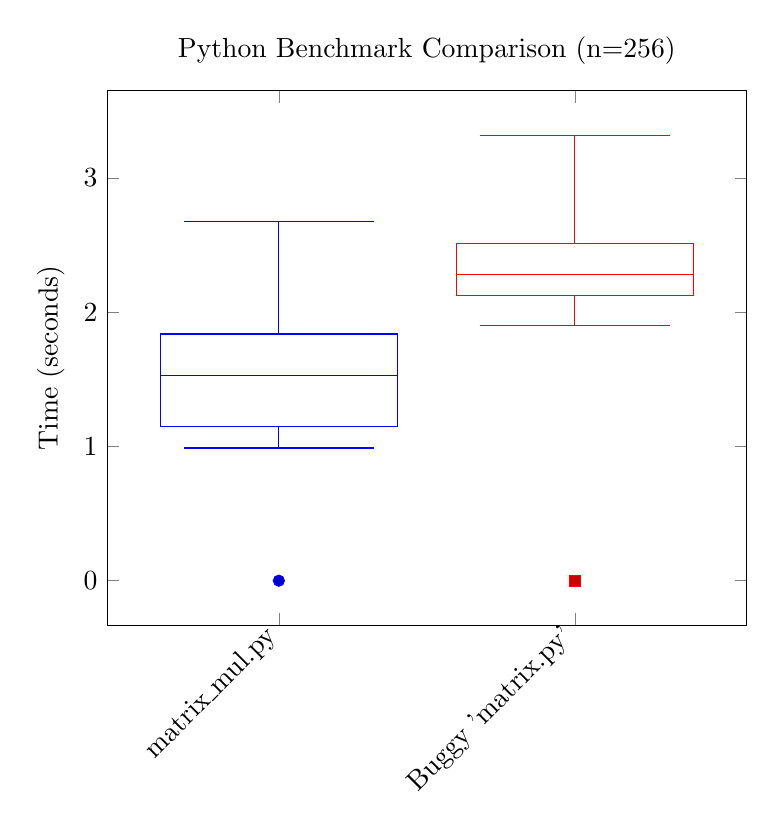
\begin{tikzpicture}
        \begin{axis}[
            title={Python Benchmark Comparison (n=256)},
            ylabel={Time (seconds)},
            boxplot/draw direction=y,
            xtick={1, 2},
            xticklabels={matrix\_mul.py, Buggy 'matrix.py'},
            x tick label style={rotate=45, anchor=east},
            width=0.8\textwidth,
        ]
        
        % Box plot for matrix_mul.py
        \addplot+[
            boxplot prepared={
                median=1.530636,
                upper quartile=1.837722,
                lower quartile=1.146174,
                upper whisker=2.677320,
                lower whisker=0.988593
            },
        ] coordinates {(1, 0)}; % Position at xtick=1

        
        % Box plot for 'matrix.py'
        \addplot+[
            boxplot prepared={
                median=2.282895,
                upper quartile=2.513846,
                lower quartile=2.121558,
                upper whisker=3.316186,
                lower whisker=1.897993
            },
        ] coordinates {(2, 0)}; % Position at xtick=2

        \end{axis}
    \end{tikzpicture}
    \caption{Box plot comparison of the two Python benchmark runs (100 runs each).}
    \label{fig:python_benchmark_comparison}
\end{figure}

\clearpage % Ensure conclusion starts on a new page if needed

The data shows a clear performance difference. The refactored and correct implementation, \texttt{matrix\_mul.py}, is significantly faster. Its median time of \textbf{1.53s} is approximately 33\% lower than the median time of \textbf{2.28s} from the original \texttt{matrix.py} script.

Interestingly, the \texttt{matrix.py} script, in addition to being incorrect, was also slower. Accessing \texttt{B[k][k]} in the inner loop likely led to a very different (and less cache-efficient) memory access pattern compared to the sequential access of \texttt{B[k][j]} in the correct version.

Furthermore, the data for \texttt{matrix\_mul.py} shows a slightly higher standard deviation (0.38s) compared to the buggy version (0.29s). This indicates greater variability in performance, which could be because the faster, more computationally-intensive code is more sensitive to other system activities or Python's garbage collection.

\section{Conclusion}
This study successfully demonstrated the process of evolving a simple script into a robust and reliable benchmark harness. By separating concerns (logic, correctness testing, performance testing), parameterizing inputs, and running multiple trials, I obtained reliable performance data.

The analysis of the results revealed that the correct \texttt{matrix\_mul.py} implementation is not only algorithmically correct but also significantly faster than the initial, flawed version. This underscores the principle that rigorous benchmarking is essential not only for optimizing performance but also for identifying and verifying the impact of algorithmic bugs.

\end{document}